Un cristal paramagnétique est formé de $N$ atomes portant chacun un moment magnétique $\overrightarrow{\mu}$. Le système, en contact avec un thermostat à la température $T$, est plongé dans un champ magnétique $\overrightarrow{B}$ orienté selon l'axe $Oz$.  On rappelle que l'énergie potentielle d'un moment magnétique $\overrightarrow{\mu}$ dans un champ $\overrightarrow{B}$ est $e=-\overrightarrow{\mu}.\overrightarrow{B}$ et on néglige les interactions entre les moments magnétiques.

\medskip

\tiret{Description classique}

Chaque moment magnétique $\overrightarrow{\mu}$ a une norme fixe $\mu$ et peut s'orienter dans une direction quelconque, repérée par les angles $\theta$ et $\phi$ des coordonnées sphériques. Un moment magnétique étant assimilé à un rotateur de moment d'inertie $\cal I$, son hamiltonien est donné par
$$
h=\frac{p_{\theta}^2}{2 {\cal I}} + \frac{p_{\phi}^2}{2 {\cal I}\sin^{2} \theta} -\mu B \cos \theta
$$

\question
Exprimer la fonction de partition $Z$ du système à l'aide de la fonction de partition $z$ d'un seul moment magnétique. Montrer que $z$ s'exprime sous la forme $z=z_{cin}z_{mag}$ où $z_{mag}$ s'exprime en fonction de $x=\beta \mu B$ et vaut 1 pour $x=0$ . Montrer que $z_{cin}$ est de la forme $z_{cin}=\frac{\cal V}{\Lambda_T^2}$ où $\cal V$ est un \og volume accessible\fg, et $\Lambda_T$ une longueur  thermique.

\question
Calculer l'énergie moyenne $\langle E \rangle$. Quelle est la contribution moyenne de l'énergie cinétique $\langle E_{\rm cin} \rangle$ ? En déduire la valeur moyenne $\langle E_{\rm mag}\rangle $ de l'énergie d'interaction avec le champ magnétique.

\question
Donner la densité de probabilité $P(\theta, \phi)$ qu'un moment magnétique pointe dans la direction donnée par les angles $\theta$ et $\phi$ à ${\rm d}\theta$ et ${\rm d}\phi$ près. Vérifier qu'en l'absence de champ magnétique la distribution de probabilité est bien isotrope. On rappelle que l'élément d'angle solide est ${\rm d}^2 \Omega= \sin \theta {\rm d} \theta {\rm d} \phi$.

\question
Calculer les valeurs moyennes $\langle \mu_x \rangle$, $\langle \mu_y \rangle$ et $\langle \mu_z \rangle$ des projections de $\overrightarrow{\mu}$ selon les axes $Ox, Oy$ et $Oz$. On exprimera $\langle \mu_z \rangle$ à l'aide de la fonction de Langevin définie par
$$
{\cal L}(x)=\frac{1}{\tanh x}-\frac{1}{x}\enspace.
$$
Tracer l'aimantation moyenne $\langle M \rangle$ en fonction de $x$.

\medskip

\tiret{Description quantique : modèle de Brillouin}

Dans le cas général, le spin porté par les atomes du cristal est un
entier ou un demi-entier $J$. La projection du moment magnétique selon
l'axe $z$ peut prendre alors $2J+1$ valeurs : $\mu_z= -g\mu_B J_z$, où
$g \simeq 2$ est le facteur de Landé et $\mu_B$ le magnéton de Bohr,
avec $J_z=-J, -J+1, \dots,J-1, J$.

\question
Calculer la fonction de partition $z$ d'un spin. On posera $x= \beta g \mu_B B$.

\noindent
On rappelle que pour une série géométrique de raison $q$ : $\displaystyle S_N=\sum_{n=0}^{N} q^n=\frac{1-q^{N+1}}{1-q}$.  

\question
En déduire la valeur moyenne $\langle \mu_z \rangle$ du moment magnétique, que l'on exprimera à l'aide de la fonction de Brillouin d'ordre $J$ donnée par
$$
{\cal B}_J(y)=\frac{2J+1}{2J} \coth \Big[\frac{2J+1}{2J}y\Big]-\frac{1}{2J}\coth \Big(\frac{y}{2J}\Big)\enspace.
$$

\question
Dans le cas particulier où $J=1/2$ et en posant $\mu = g\mu_B J$, que devient l'expression de $\langle \mu_z \rangle$. Commenter ce résultat. 

\question
On donne au voisinage de l'origine  ${\cal B}_J(y)= \frac{J+1}{3J} y+O(y^3)$. Montrer qu'à haute température, on retrouve à nouveau la loi de Curie, mais qu'à faible température, on est loin du résultat classique obtenu dans la partie précédente (sauf dans la limite des grandes valeurs de $J$).

\begin{figure}[h]
\begin{center} 
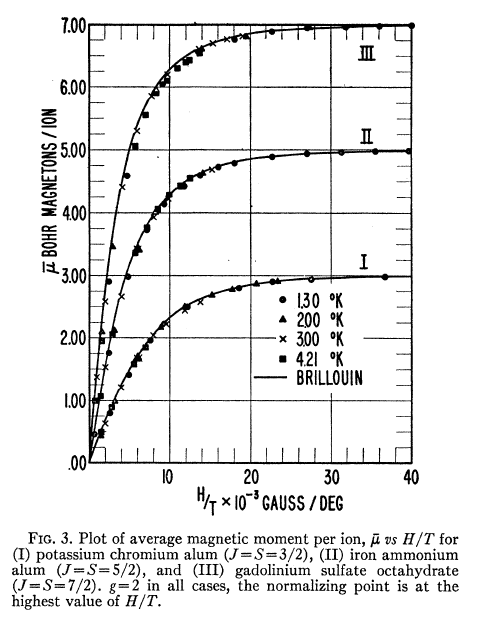
\includegraphics[height=.5\textwidth]{../Fig/Brillouin}
\caption{\it Moment magnétique moyen par ion (en unité du magnéton de Bohr) en fonction de $B/T$ pour certains sels paramagnétiques : (I) Cr$^{3+}$, (II) Fe$^{3+}$ et (III) Gd$^{3+}$.  Les points sont les données expérimentales et les courbes en traits pleins correspondent aux résultats obtenus en utilisant des fonctions de Brillouin [tirée de W. E. Henry, Phys. Rev. \textbf{88}, 559 (1952)]. Pourriez vous estimer la valeur de $J$ pour chaque ion ?}
\end{center} 
\end{figure}
